%%%% Better Poster latex template example v1.0 (2019/04/04)
%%%% GNU General Public License v3.0
%%%% Rafael Bailo
%%%% https://github.com/rafaelbailo/betterposter-latex-template
%%%% 
%%%% Original design from Mike Morrison
%%%% https://twitter.com/mikemorrison

\documentclass[a0paper,fleqn]{betterposter}

%%%% Uncomment the following commands to customise the format

%% Setting the width of columns
% Left column
%\setlength{\leftbarwidth}{0.25\paperwidth}
% Right column
%\setlength{\rightbarwidth}{0.25\paperwidth}

%% Setting the column margins
% Horizontal margin
%\setlength{\columnmarginvertical}{0.05\paperheight}
% Vertical margin
%\setlength{\columnmarginhorizontal}{0.05\paperheight}
% Horizontal margin for the main column
%\setlength{\maincolumnmarginvertical}{0.15\paperheight}
% Vertical margin for the main column
%\setlength{\maincolumnmarginhorizontal}{0.15\paperheight}

%% Changing font sizes
% Text font
%\renewcommand{\fontsizestandard}{\fontsize{28}{35} \selectfont}
% Main column font
%\renewcommand{\fontsizemain}{\fontsize{28}{35} \selectfont}
% Title font
%\renewcommand{\fontsizetitle}{\fontsize{28}{35} \selectfont}
% Author font
%\renewcommand{\fontsizeauthor}{\fontsize{28}{35} \selectfont}
% Section font
%\renewcommand{\fontsizesection}{\fontsize{28}{35} \selectfont}

%% Changing font sizes for a specific text segment
% Place the text inside brackets:
% {\fontsize{28}{35} \selectfont Your text goes here}

%% Changing colors
% Background of side columns
%\renewcommand{\columnbackgroundcolor}{black}
% Font of side columns
%\renewcommand{\columnfontcolor}{gray}
% Background of main column
%\renewcommand{\maincolumnbackgroundcolor}{empirical}
%\renewcommand{\maincolumnbackgroundcolor}{theory}
%\renewcommand{\maincolumnbackgroundcolor}{methods}
%\renewcommand{\maincolumnbackgroundcolor}{intervention}
% Font of main column
%\renewcommand{\maincolumnfontcolor}{gray}
\DeclareFontFamily{U}{skulls}{}
\DeclareFontShape{U}{skulls}{m}{n}{ <-> skull }{}
\newcommand{\skull}{\text{\usefont{U}{skulls}{m}{n}\symbol{'101}}}

\begin{document}	
\betterposter{
%%%%%%%% MAIN COLUMN

\maincolumn{
%%%% Main space

\textbf{Main finding} goes here, \\
translated into \textbf{plain English}.\\
\textbf{Emphasize} the important words.
}{
%%%% Bottom space

%% QR code
\qrcode{images/qr-code.png}{images/smartphone}{
\textbf{Take a picture} to \\
download the full paper
}
% Smartphone icon
% Author: Freepik
% Retrieved from: https://www.flaticon.com/free-icon/smartphone_65680

%% Compact QR code (comment the previous command and un-comment this one to switch)
%\compactqrcode{images/qr-code.png}{
%\textbf{Take a picture} to
%\\download the full paper
%}

}

}{
%%%%%%%% LEFT COLUMN

\title{The Title}
\author{Author 1}
\author{Author 2}
\author{Author 3}
\author{Author 4}
\author{Author 5}
\author{Author 6}
\institution{UCLA Statistics}

\section{Introduction}
Here is an itemized list:
\begin{itemize}
\item The first item.
\item The second item.
\item The third item.
\end{itemize}

\section{A Diagram}
Here is a diagram:
\begin{center}
% Linear regression
% Author: Henri Menke
% Retrieved from: http://www.texample.net/tikz/examples/linear-regression/
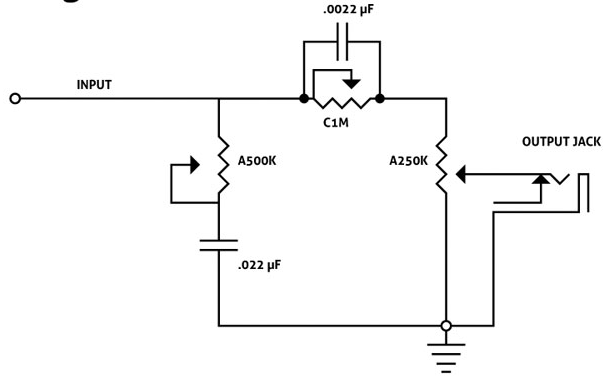
\includegraphics[width=\textwidth]{images/diagram1.png}
\end{center}

\section{Fundamental Theorem\\of Calculus}
If $f$ is continuous on the closed interval $[a,b]$ and $F$ is the indefinite integral of $f$ on $[a,b]$, then
\begin{equation}
\int_a^b f(x)\,\mathrm{d}x = F(b)-F(a).
\end{equation}

\section{Conclusion}
Perhaps this will work for you!

%% This fills the space between the content and the logo
%\vfill

%% Institution logo
%
\includegraphics[width=\textwidth]{images/DeptLogo.png}\\

}{
%%%%%%%% RIGHT COLUMN

Here you can add \textbf{supplementary material}. For instance, more text:\\
Lorem ipsum dolor sit amet, consectetur adipiscing elit. In vitae sapien nec orci auctor lacinia. Aenean pretium ante fringilla consequat posuere. Quisque tempus libero magna, et vehicula nisi venenatis at. Nam cursus turpis et augue maximus sollicitudin. Etiam eleifend tristique pretium. Praesent odio leo, posuere vitae eros ut, finibus pellentesque lorem. Morbi vel ultrices enim. Etiam pulvinar justo iaculis purus tristique, in molestie erat efficitur. Nullam non justo leo. Suspendisse id sagittis lorem. In ac dolor at dui malesuada placerat. Aliquam quis quam et urna varius pellentesque.



\section{Alternative Abstract}
\begin{center}
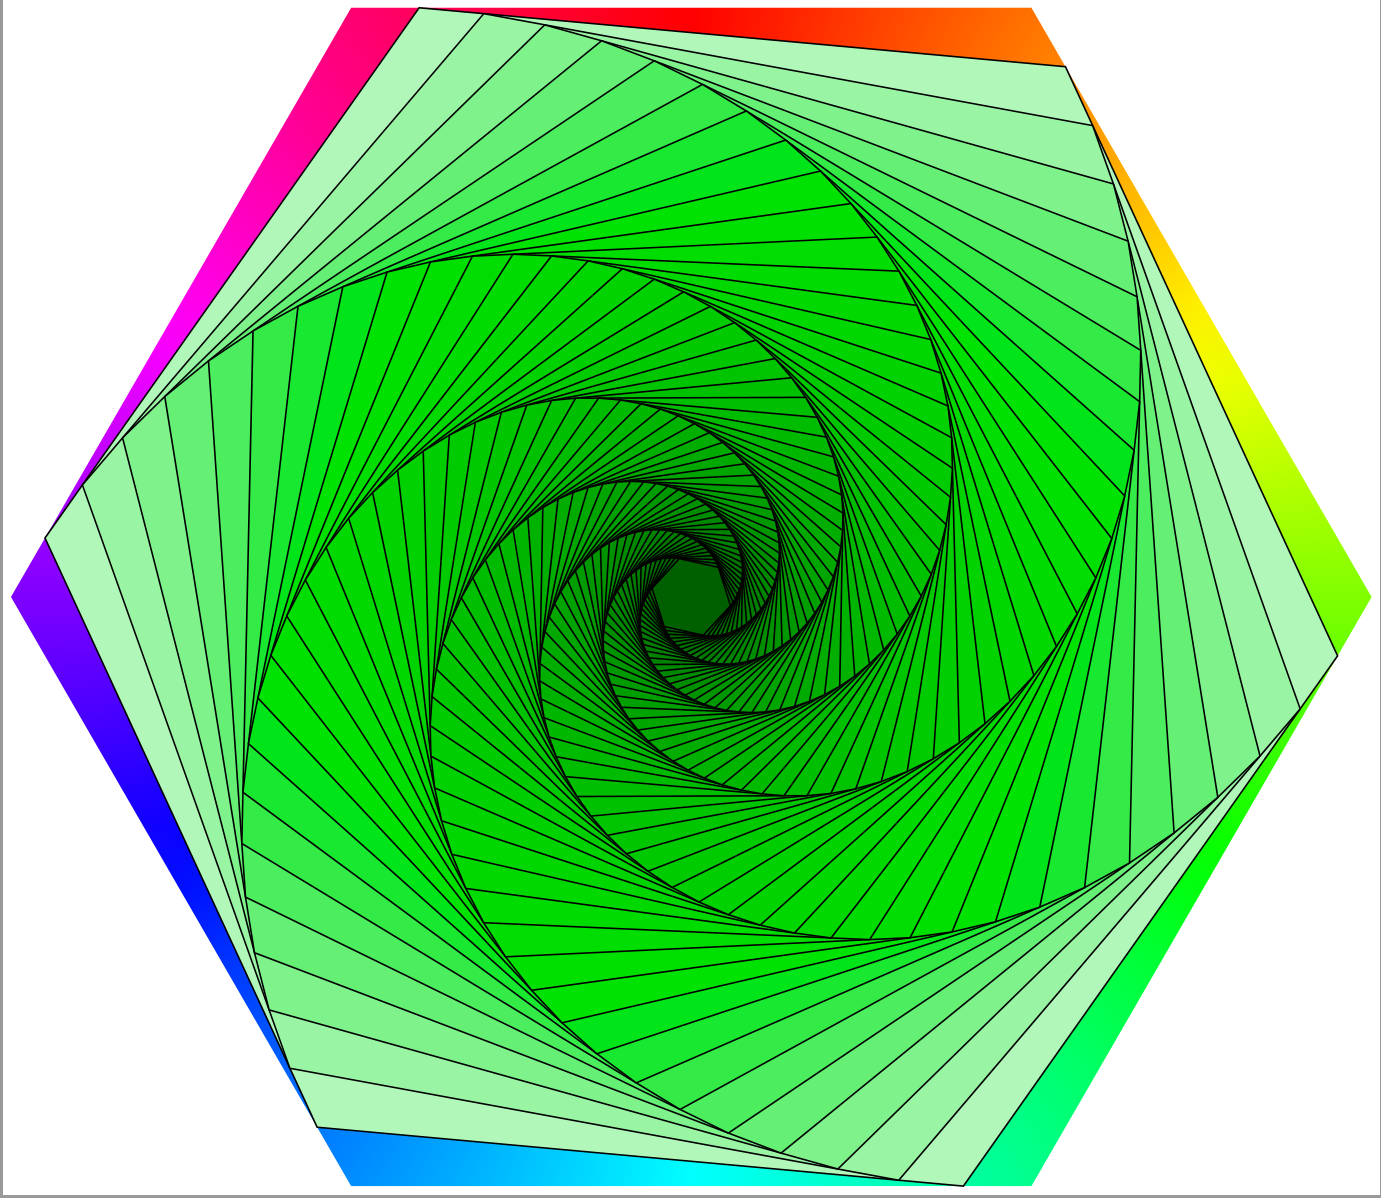
\includegraphics[width=\textwidth]{images/tyre.png}
\end{center}

\section{Haiku by Professor Zes}
\begin{center}
    Stat roles everywhere\\
    Your degree the difference\\
        Cookie Monster growl \\
        $\skull$
\end{center}
%% This fills the space between the content and the logo
\vfill

%% Institution logo

\includegraphics[width=\textwidth]{images/UCLA_ds_001.png}\\

}

\end{document}
